\section*{Схема экспериментальной установки}

Схема экспериментальной установки изображена на рисунке:

\begin{figure}[H]
	\centering
	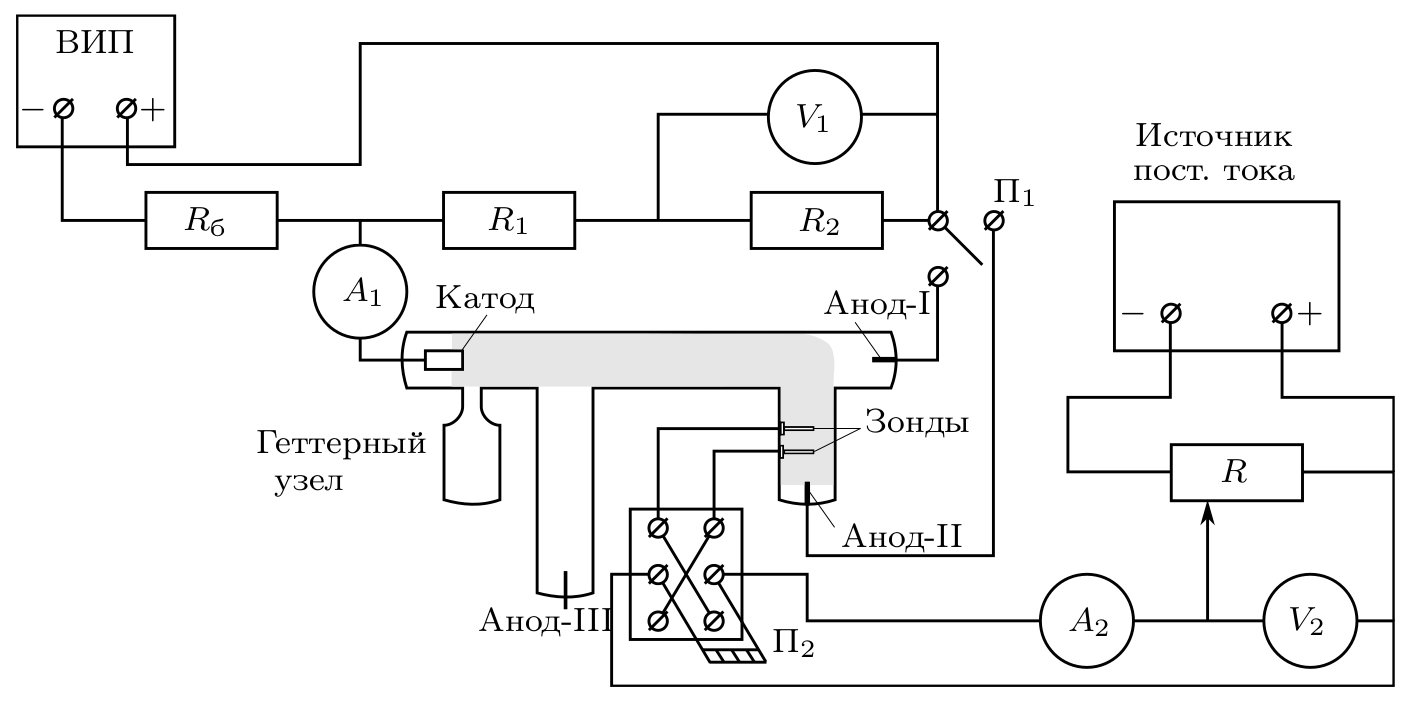
\includegraphics[width=1\textwidth]{../res/exp scheme.png}
\end{figure}

Установка состоит из стеклянной газоразрядной трубки, в которой находится катод и три анода. В данной работе анод 3 не используется. Трубка наполнена изотопом неона $^{22}Ne$ при давлении 2 мм рт.ст. Катод и один из анодов с подключаются к высоковольтному источнику питания (ВИЧ) через балластный резистор $R_б \approx 450 \; кОм$. Анод 1 и 2 можно подключать к ВИЧ через переключатель $П_1$. Миллиамперметр $А_1$ измеряет ток между анодом и катодом, а цифровой вольтметр $V_1$ измеряет напряжение в газоразрядной трубке. Вольтметр $V_1$ подключен через делитель напряжения с коэффициентом $K = 10$. 

Во второй части работы исследуются характеристики плазмы с помощью двух зондов. Зонды изготовлены из молибденовой проволоки диаметром $d = 0,2 \; мм$, длиной $l = 5,2 \; мм$. С помощью источника постоянного тока на зонды подается ток, который измеряется миллиамперметром $A_2$. Напряжение на зондах измеряется вольтметром $V_2$. Для регулировки напряжения используется реостат $R$.

